\documentclass[twocolumn,superscriptaddress,showpacs,preprintnumbers,amsmath,amssymb,prl]{revtex4}
\usepackage{graphicx}
\usepackage{dcolumn,xcolor,ulem}
\usepackage{amsmath} 
\usepackage{amssymb}
\usepackage{amsfonts}
\usepackage{bm}
\usepackage[latin1]{inputenc}
%\usepackage{mathrsfs}

\newcommand{\cor}[1]{\textcolor{red}{#1}}
\newcommand{\change}[1]{\textcolor{blue}{#1}}
\newcommand\gp{\dot\gamma}
\newcommand\gl{\gamma_{\rm loc}}
\newcommand\gpm{\dot\gamma_{\rm min}}
\newcommand\taum{\tau_{\rm min}}

\newcommand{\ti}[1]{\textbf{\color{blue}#1}} % remarques de Thibaut
\newcommand{\titi}[1]{\sout{\textbf{\color{blue}#1}}} % remarques de Thibaut

\begin{document}

%\widowpenalty=1000
%\clubpenalty=1000
%\preprint{APS/123-QED}

 \title{Creep and fracture of a protein gel under stress}

\author{M.~Leocmach}
\email{mathieu.leocmach@ens-lyon.fr}
\affiliation{Universit\'e de Lyon, Laboratoire de Physique, \'Ecole Normale Sup\'erieure de Lyon, CNRS UMR 5672, 46 All\'ee d'Italie, 69364 Lyon cedex 07, France}
\author{C.~Perge}
\affiliation{Universit\'e de Lyon, Laboratoire de Physique, \'Ecole Normale Sup\'erieure de Lyon, CNRS UMR 5672, 46 All\'ee d'Italie, 69364 Lyon cedex 07, France}
\author{T.~Divoux}
%\email{divoux@crpp-bordeaux.cnrs.fr}
\affiliation{Centre de Recherche Paul Pascal, CNRS UPR 8641 - 115 avenue Schweitzer, 33600 Pessac, France}
\author{S.~Manneville}
\affiliation{Universit\'e de Lyon, Laboratoire de Physique, \'Ecole Normale Sup\'erieure de Lyon, CNRS UMR 5672, 46 All\'ee d'Italie, 69364 Lyon cedex 07, France}

\date{\today}

\begin{abstract}
Biomaterials such as protein or polysaccharide gels are known to behave qualitatively as soft solids and to rupture under an external load. Combining optical and ultrasonic imaging to shear rheology we show that the failure scenario of a protein gel is reminiscent of brittle solids: after a primary creep regime characterized by a macroscopically homogeneous deformation and a power-law behavior which exponent is fully accounted for by linear viscoelasticity, fractures nucleate and grow logarithmically perpendicularly to shear, up to the sudden rupture of the gel. A single equation accounting for those two successive processes nicely captures the full rheological response. The failure time follows a decreasing power-law with the applied shear stress, similar to the Basquin law of fatigue for solids. These results are in excellent agreement with recent fiber-bundle models that include damage accumulation on elastic fibers and exemplify protein gels as model, brittle-like soft solids.
\end{abstract}

\pacs{}
\maketitle

Biogels formed through the self-association of polysaccharide coils, collagen, actin filaments or attractive globular proteins play a major role in biochemistry and microbiology \cite{Viovy:2000}, biological networks and cell mechanics \cite{Stricker:2010} as well as in food science \cite{Mezzenga:2005}. These biomaterials all behave as elastic solids under small deformations but display remarkable nonlinear behavior generally featuring stress- or strain-stiffening \cite{Gardel:2004} and fractures prior to irreversible rupture \cite{Bonn:1998,Baumberger:2006}. Irreversibility stems from the existence of an external control parameter, e.g. temperature or pH in the case of thermoreversible or acid-induced gels respectively. This makes such biogels fundamentally different from other soft glassy materials such as emulsions, colloidal gels and glasses that can be rejuvenated by shear \cite{Cloitre:2000,Caton:2008,Divoux:2011,Siebenburger:2012} or transient networks where fractures spontaneously heal \cite{Tabuteau:2009,Skrzeszewska:2010}. So far, huge effort has been devoted to the design of protein gels with specific properties and textures at rest \cite{Dickinson:2006,Gibaud:2012}. However, their mechanical behavior deep into the nonlinear regime has only been partially addressed \cite{vanVliet:1995,Pouzot:2006} and several fundamental issues remain unexplored such as the spatially resolved rupture scenario or the physical relevance of the analogy with brittle failure in hard solids.

%%%%%%%%%%%%
\begin{figure}
\centering
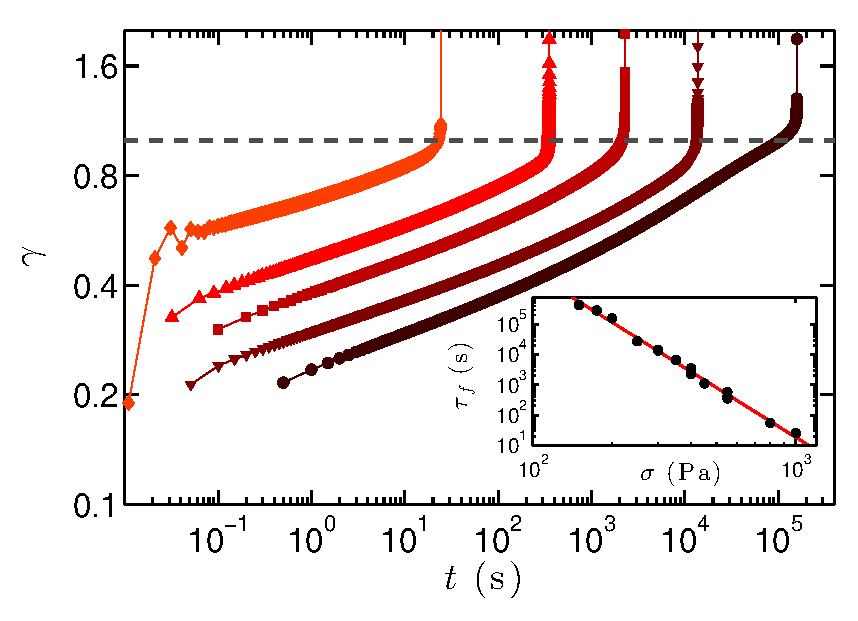
\includegraphics[width=7cm]{Fig1.eps}
\caption{(color online) Strain response $\gamma(t)$ in a 4\%~wt. casein gel acidified with 1\%~wt. GDL for an imposed shear stress $\sigma=200$ (\textcolor{red!25!black}{$\bullet$}), 300 (\textcolor{red!50!black}{$\blacktriangledown$}), 400 (\textcolor{red!75!black}{$\blacksquare$}), 550 (\textcolor{red}{$\blacktriangle$}) and 1000~Pa (\textcolor{orange!50!red}{$\blacklozenge$}) from right to left. The gap width is 1~mm. Gray dashes show $\gamma=1$. Inset: failure time $\tau_f$ vs $\sigma$. The red line is the best power-law fit $\tau_f=A\sigma^{-\beta}$ with $\beta=5.45\pm 0.05$ and $A=40.6\pm 0.5$~s.Pa$^\beta$.
\label{fig1}}
\end{figure} 
%%%%%%%%%%%%

In this Letter we report on stress-induced fracture in protein gels by means of creep experiments coupled to optical and ultrasonic imaging. Gels formed by slow acidification of a sodium caseinate solution display fractures under large strain at fixed low pH values \cite{vanVliet:1995,Lucey:1998}, which makes them perfect candidates to quantify the rupture of soft solids and tackle the above-mentioned issues. We demonstrate that under an external load, these casein gels display brittle-like failure that results from two successive physical processes: (i) a primary creep regime characterized by a macroscopically homogeneous strain field where dissipation is dominated by viscous flow through the gel matrix and (ii) the irreversible nucleation and growth of fractures leading to gel failure. Our results are in full agreement with the predictions of some recent fiber-bundle models and hint to universal features of failure common to both soft and hard solids.

%%%%%%%%%%%%
\begin{figure}
\centering
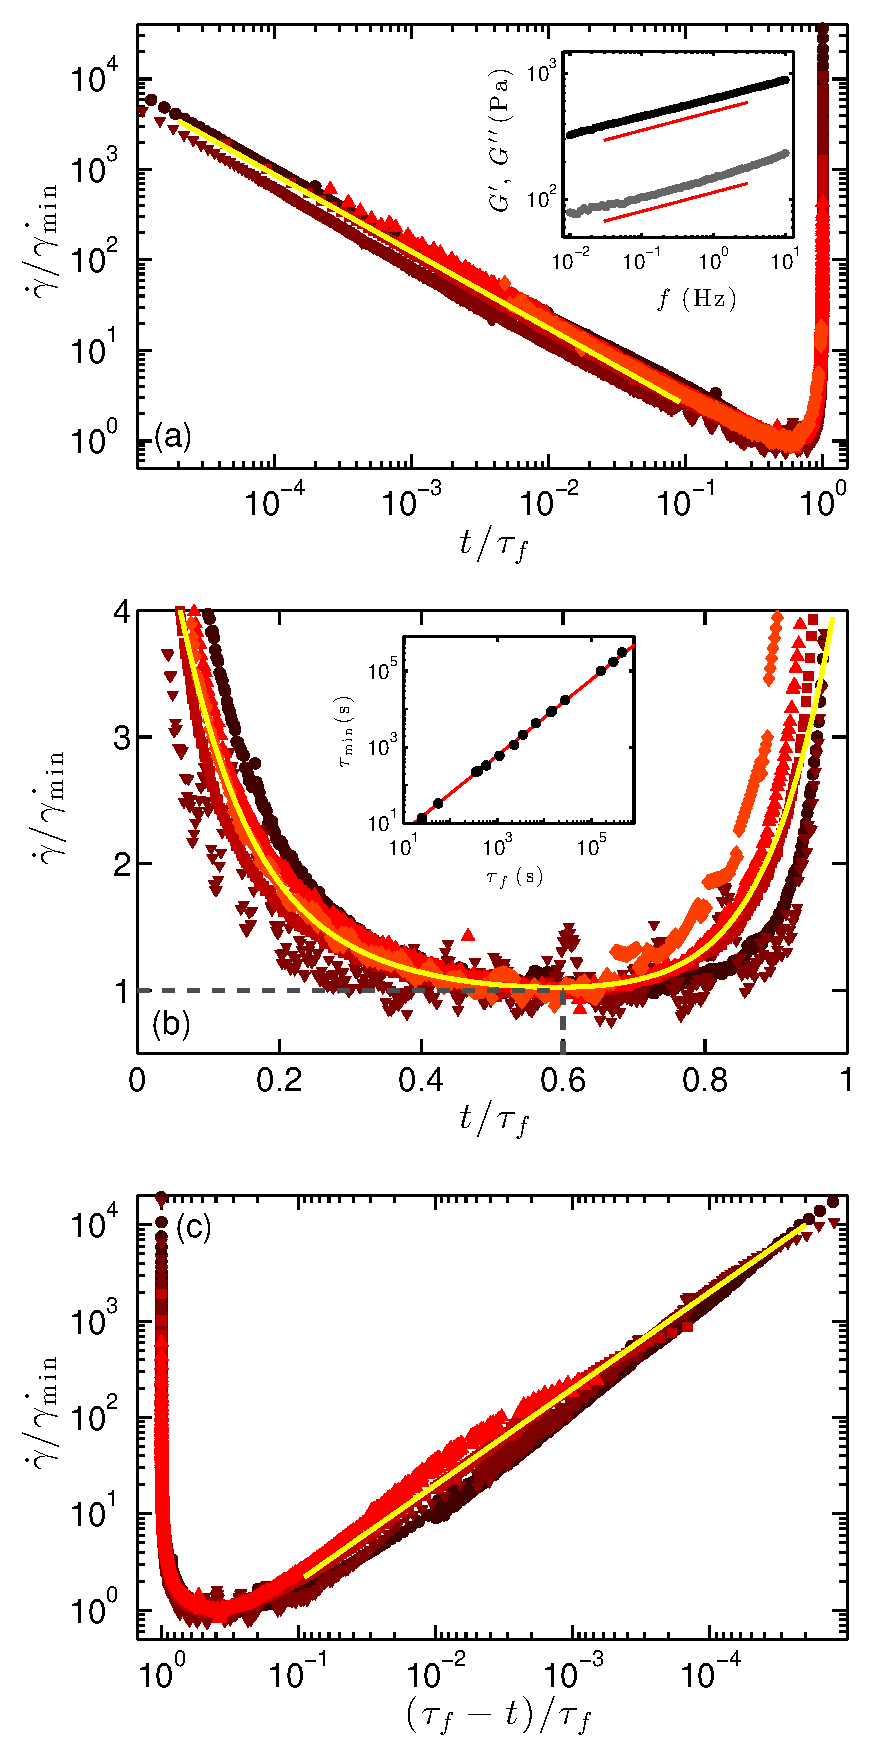
\includegraphics[width=7cm,clip]{Fig2.eps}
\caption{(color online) Normalized shear rate responses $\gp(t)/\gpm$ corresponding to the data of Fig.~\ref{fig1} and plotted so as to emphasize the three successive regimes. $\gpm$ is the minimum shear rate reached at $\taum$ (see text and Suppl. Fig.~2). The yellow line shows the master curve inferred from fitting $\gp(t)$ by Eq.~(\ref{e.fit}) with $\alpha=0.85$, leading to $\lambda=0.378\pm 0.002$ and $\mu=0.187\pm 0.002$. (a)~Primary creep: $\gp(t)/\gpm$ vs $t/\tau_f$ in logarithmic scales. Inset: Linear viscoelastic moduli $G'$ (top) and $G''$ (bottom) as a function of frequency $f$ for a strain amplitude of 0.1\%. Red lines are power laws $G'\sim G''\sim f^{0.15}$. (b)~Secondary creep: $\gp(t)/\gpm$ vs $t/\tau_f$ in linear scales. Gray dashes show the minimum of Eq.~(\ref{e.fit}) reached at $\taum=0.556\tau_f$. Inset: $\taum$ vs $\tau_f$. The red line is $\taum=0.56\tau_f$. (c)~Tertiary creep: $\gp(t)/\gpm$ vs $(\tau_f-t)/\tau_f$ in logarithmic scales with a reversed horizontal axis.\label{fig2}}
\end{figure} 
%%%%%%%%%%%%

Gels are prepared by dissolving sodium caseinate powder (Firmenich) at 4\% wt. in deionized water under gentle mixing at 35$^{\circ}$C and 500~rpm. To induce gelation, 1\% wt. glucono-$\delta$-lactone (GDL) in powder (Firmenich) is dissolved in the solution and its hydrolysis progressively lowers the pH over the course of 8~hours [Fig.~\ref{suppfig1}(a) in the Supplemental Material]. While still liquid, the solution is poured into the gap of a polished Plexiglas Couette cell immersed into a temperature-controlled water tank at 25.0$\pm$0.1$^{\circ}$C \cite{note}. Rheological data are recorded during gel formation by a stress-controlled rheometer through small amplitude oscillatory shear at frequency $f=1$~Hz (Fig.~1 in the Supplemental Material) \cite{note}. Gelation is complete when the elastic ($G'$) and viscous ($G''$) moduli reach a plateau with $G'\gg G''$. A constant stress $\sigma$ is then applied to the sample from time $t=0$ and the subsequent strain response $\gamma(t)$ is monitored. Images of the gel are recorded simultaneously to the rheology (Logitech Webcam Pro 9000). The local velocity and strain fields can also be imaged in the gradient--vorticity plane $(r,z)$ simultaneously to rheology by a custom-made ultrasonic scanner detailed in \cite{Gallot:2013}. In this case, prior to acidification, the sodium caseinate solution is seeded with acoustic tracers here 3\% wt. polyamide spheres (Orgasol 2002 ES3 NAT 3, Arkema, diameter 30~$\mu$m, density 1.02) that do not modify the final gel properties [Fig.~\ref{suppfig1}(b) in the Supplemental Material]. Failure being irreversible, each creep experiment requires to prepare a fresh sample in-situ.  

Under a constant applied shear stress $\sigma$, the global strain $\gamma(t)$ displays a robust time dependence (Fig.~\ref{fig1}): $\gamma(t)$ slowly grows with time up to $\gamma \sim 1$ then accelerates until the gel fails at a well-defined time $\tau_f$. These three successive steps are better highlighted in Fig.~\ref{fig2} by focusing on the global shear rate $\gp(t)$. Figures~\ref{fig3} and \ref{fig4} gather the results from {\it local} measurements and are discussed below together with each of the successive regimes inferred from {\it global} data. Note that these failure dynamics do not qualitatively depend on geometry nor on system composition (see Movie~1 in the Supplemental Materials).

%%%%%%%%%%%%
\begin{figure*}[t]
\centering
\includegraphics[width=17.5cm,clip]{Fig3.eps}
\caption{(color online) Ultrasonic images (left) and direct visualization of the Couette cell (right) recorded simultaneously at various times in the primary [(a)~$t/\tau_f=0.02$], secondary [(b)~$t/\tau_f=0.57\simeq\taum/\tau_f$] and tertiary  [(c) $t/\tau_f=0.93$ and (d) 0.99] creep regimes. Ultrasonic images are azimuthal velocity maps $v(r,z,t)$ computed by averaging over 4~s and coded using the linear color levels shown below the images. Their position relative to the picture of the cell reflects the actual arrangement of the ultrasonic probe along the vertical direction $z$. The gap width is 2~mm and $r$ is the radial distance to the inner rotating cylinder. Experiment performed on a 4\%~wt. casein gel seeded with 3\%~wt. polyamide spheres and acidified with 1\%~wt. GDL under $\sigma=300$~Pa. See also Movie~2 in the Supplemental Material.
\label{fig3}}
\end{figure*} 
%%%%%%%%%%%%

As seen in the inset of Fig.~\ref{fig1}, the failure time $\tau_f$ sharply decreases as a power-law of $\sigma$ with an exponent $\beta\simeq 5.5$. $\tau_f$ further allows us to rescale all the shear rate data $\gp(t)$ onto the single master curve of Fig.~\ref{fig2}(a) by plotting $\gp/\gp_{\rm min}$ vs $t/\tau_f$, where $\gp_{\rm min}$ is the minimum shear rate reached at a time $\tau_{\rm min}$ [see also Fig.~\ref{suppfig2} in the Supplemental Material for the original $\gp(t)$ data]. On about four decades for $t\lesssim 0.1\tau_f$, the shear rate decreases as a power-law $\gp(t)\sim t^{-\alpha}$ with $\alpha=0.85\pm 0.04$. This is strongly reminiscent of the {\it primary creep} observed in solids and referred to as Andrade creep \cite{Andrade:1910,Miguel:2002,Nechad:2005,Rosti:2010}. Interestingly, here, the exponent can be inferred from linear viscoelasticity. Indeed casein gels display a power-law rheology $G'(f)\sim G''(f)\sim f^{0.15}$ [inset of Fig.~\ref{fig2}(a)], which corresponds to a compliance $J(t)\equiv\gamma(t)/\sigma\sim t^{0.15}$ in the linear deformation regime \cite{Tschoegl:1989}. This nicely corresponds to the observed $\gp(t)\sim t^{-0.85}$. Moreover ultrasonic imaging reveals velocity and strain fields averaged over the vertical direction $z$ that linearly decrease with the radial position $r$ within the gap [Fig.~\ref{fig4}(a-b)] with insignificant $z$-dependence [Fig.~\ref{fig3}(a, left)] and no slippage at the Plexiglas walls. Together with direct visualization [Fig.~\ref{fig3}(a)], these local measurements demonstrate that during primary creep there is no macroscopic strain localization or fracture, although we cannot rule out microscopic rearrangements below the available spatial ($\sim10~\mu$m) and temporal ($\sim1$~s) resolutions.

For $0.1\lesssim t/\tau_f\lesssim 0.9$, $\gp(t)$ departs from power-law behavior and goes through a minimum value at time $\tau_{\rm min}= (0.56\pm0.04)\tau_f$ independently of the applied stress [Fig.~\ref{fig2}(b) and inset] as similarly reported for metals \cite{Sundararajan:1989}, solid composite materials \cite{Nechad:2005} and fiber-bundle models (FBMs) \cite{Kovacs:2008,Jagla:2011}. This linearity between $\tau_{\rm min}$ and $\tau_f$, also known as the Monkman-Grant relation \cite{Monkman:1956}, allows one to ``predict'' the failure time from the intermediate-time response. During this {\it secondary creep} regime, regularly-spaced cracks nucleate from the top and bottom edges of the Couette cell and start growing perpendicular to the applied stress [Fig.~\ref{fig3}(b), see also Movie~2 in the Supplemental Material]. These macroscopic fractures are invaded with water expelled from the surrounding gel matrix. Although fractures have not yet entered the ultrasonic region of interest, velocity maps become heterogeneous along the $z$ direction [Fig.~\ref{fig3}(b, left)] and display intermittent fluctuations [Fig~\ref{fig4}(c,d)]. The level of these fluctuations, which can also be seen on the global response for the same applied stress [\textcolor{red!50!black}{$\blacktriangledown$} in Fig.~\ref{fig2}(b)], is poorly reproducible and stress-dependent. Such intermittency may arise from crack growth outside the region of interest which induces long-range elastic deformation propagating across the sample mainly along the vertical direction [see the lower level of fluctuations along the radial direction in Fig~\ref{fig4}(d)].

In the {\it tertiary creep} regime, for $t\gtrsim 0.9\tau_f$, the shear rate increases by more than four orders of magnitude and diverges as $(\tau_f-t)^{-1}$ [Fig.~\ref{fig2}(c)]. This finite-time singularity corresponds to the final growth of the fractures along the vorticity direction $z$ as they accelerate and eventually meet in the middle of the Couette cell at time $\tau_f$ [Fig.~\ref{fig3}(c-d)]. Ultrasonic velocity maps directly correlate with the crack growth and reveal the complex structure of the displacement field at the tip and around the fracture. In particular, Fig.~\ref{fig3}(d, left) suggests that the fracture is initiated at the inner cylinder at $r=0$ and the presence of large positive and negative velocities in the vicinity of the crack tip is indicative of strong compression and recoil of the gel matrix. Finally, the fracture length $\ell(t)$ is observed to grow logarithmically with $(\tau_f-t)$ upon approaching $\tau_f$ [Fig~\ref{fig4}(d)]. In other words one has ${\rm d}\ell/{\rm d}t\sim\gp(t)\sim (\tau_f-t)^{-1}$, which indicates that the global shear rate is linked to fracture-induced displacements.

%%%%%%%%%%%%
\begin{figure*}
\centering
\includegraphics[width=17.5cm,clip]{Fig4.eps}
\caption{(color online) (a)~Local velocity $\langle v(r,z,t)\rangle_z$ and (b)~local strain field $\langle\gl(r,z,t)\rangle_z$ averaged over the vertical direction $z$ at various times during primary creep: $t/\tau_f=1.9\,10^{-3}$ ($\bullet$), $1.7\,10^{-2}$ (\textcolor{blue}{$\blacktriangledown$}) and 0.15 (\textcolor{red}{$\blacksquare$}). Solid lines are linear profiles. (c)~Spatiotemporal diagram of the local velocity $\langle v(r,z,t)\rangle_r$ averaged over the radial direction $r$ and plotted in linear color levels as a function of $z$ and $t/\tau_f$. (d)~Standard deviation $\delta_z v(t)$ of $\langle v(r,z,t)\rangle_r$ taken over the vertical direction $z$ (thick black line) together with corresponding standard deviation $\delta_r v(t)$ computed over the radial direction $r$ on the $z$-average $\langle v(r,z,t)\rangle_z$ (thin red line). (e)~Fracture length $\ell(t)$ vs $(\tau_f-t)/\tau_f$ as inferred from direct visualization ($\bullet$, average over 6 different fractures, error bars show the standard deviation) and from ultrasonic imaging ($\circ$) and normalized by the height $H$ of the Couette cell. Gray dots show the visualization data for the longest fracture which leads to the failure of the sample at $\tau_f$. Red lines are the best fits $\ell(t)=a+b\log(1-t/\tau_f)$ to the visualization data. Same experiment as in Fig.~\ref{fig3} and Supplemental Movie~2.
\label{fig4}}
\end{figure*} 
%%%%%%%%%%%%

Finally, we emphasize that the Andrade-like creep and the crack growth are two  physical processes that effectively superimpose to yield the global rheological response. Indeed, as seen from the yellow line in Fig.~\ref{fig2}, the master curve $\gp(t)/\gp_{\rm min}$ vs $t/\tau_f$ is perfectly fitted by:
%the master curve $\tilde{\gp}(t)=\gp(t)/\gp_{\rm min}$ vs $\tilde{t}=t/\tau_f$ is perfectly fitted by:
\begin{equation}
\frac{\gp(t)}{\gp_{\rm min}}=\lambda \left(\frac{t}{\tau_f}\right)^{-\alpha}+ \frac{\mu}{1-t/\tau_f}\,,
%\tilde{\gp}(\tilde{t})=\lambda \tilde{t}^{-\alpha}+ \frac{\mu}{1-\tilde{t}}\,,
\label{e.fit}
\end{equation}
with only two adjustable parameters $\lambda$ and $\mu$ once $\alpha=0.85$ is fixed. The remarkable collapse of the whole data set to such a simple equation allows us to interpret the secondary creep regime as a mere crossover from creep to crack growth.

Let us now summarize and discuss the most prominent results of this Letter. First we have shown that casein gels display a remarkable failure scenario similar to that of brittle solids and characterized by the same three successive creep regimes. Here, the power-law exponent of the primary creep [$\gp(t)\sim t^{-\alpha}$ with $\alpha=0.85\pm 0.04$] is fully accounted for by linear viscoelasticity and local measurements consistently display a homogeneous bulk deformation. Such a link between creep and viscoelasticity is shared by other biopolymer gels with power-law rheology \cite{Gobeaux:2010,Jaishankar:2013} as well as hard-sphere-like colloidal glasses \cite{Siebenburger:2012}. To better understand this link, additional creep and recovery tests were performed within the primary regime (Figs.~3 and 4 in the Supplemental Material). Successive loading/unloading sequences on a fresh sample show that (i)~the strain is not fully recovered by a few percents, (ii)~the viscoelastic properties of the material are unaltered and (iii)~strain responses are indistinguishable from one test to another. This strongly suggests that the small irreversibility observed in the primary regime mainly stems from viscous dissipation (which accounts for the nonzero viscous modulus $G''$) due to the solvent flow within the gel fibrous matrix and involves only a minute amount of local damage of the gel network. Protein gels thus appear to experience a {\it kinetically} reversible primary creep, i.e. dominated by viscous dissipation rather than by plasticity.

The logarithmic fracture growth in the tertiary creep regime constitutes our second important result. Such an evolution is also commonly reported in disordered solid materials displaying brittle rupture and interpreted in the framework of Griffith-like models based on global or local energy barriers \cite{Vanel:2009}. However these approaches all predict exponential scalings for $\tau_f(\sigma)$ while our data are best fitted by the decreasing power-law $\tau_f \sim \sigma^{-\beta}$ with $\beta=5.45\pm 0.05$ [inset of Fig.~\ref{fig1}]. This last key result suggests that thermally activated crack growth is not relevant to the present soft solid. Rather the power-law scaling is strikingly reminiscent of the Basquin law of fatigue found for a variety of heterogeneous or cellular materials under cyclic deformation \cite{Kun:2007,Basquin:1910,Kohout:2000}. Basquin law has also been recently predicted for creep experiments by FBMs that combine elastic fibers with a local yield strain and take into account damage accumulation \cite{Kun:2007,Halasz:2012}. Interestingly assuming damage accumulation to be proportional to $\sigma^\gamma$ directly leads to Basquin law with $\beta=\gamma$ and large values of $\gamma$, typically larger than 5 as found here for $\beta$, lead to macroscopic cracks due to the simultaneous rupture of a large number of fibers \cite{Halasz:2012}. More generally FBMs under elongational load predict three successive creep regimes exactly alike Fig.~\ref{fig2} with similar proportionality between $\tau_{\rm min}$ and $\tau_f$ and finite-time singularity \cite{Nechad:2005,Jagla:2011}. This highlights the relevance of FBMs in the context of creep in protein gels, whose microstructure indeed appears to be formed of strands \cite{Kalab:1983,Roefs:1990}, but also urges to study FBMs in shear geometries to check whether they would be able to predict fracture growth as observed here.

To conclude, the present time- and space-resolved study exemplifies protein gels as model, brittle-like soft solids. Prompted by the remarkable simplicity of Eq.~(\ref{e.fit}) that encompasses Andrade creep, the Monkman-Grant relation and finite-time singularity within a single equation, future modeling will undoubtedly focus on the microscopic ingredients needed to predict quantitatively the Monkman-Grant prefactor and the Basquin exponent $\beta$. The next experimental step consists in a statistical study of the fluctuations associated to crack nucleation and growth as well as a systematic investigation of other systems in order to check for universality in the irreversible creep rupture of soft solids in general and of biogels such as actin, alginate or agar gels in particular. Such a study is expected to have important implications in understanding the behavior of biomaterials under extreme stress conditions.

\begin{acknowledgments}
The authors thank M. Alava, T.~Gibaud, S.~Lindstr\"om, G.~H.~McKinley and N.~Taberlet for fruitful discussions, M.~Kal\'ab for kindly providing us with unobtainable references, and A.~Parker at Firmenich for precious advice and for providing the casein and GDL. This work was funded by the Institut Universitaire de France and by the European Research Council under the European Union's Seventh Framework Programme (FP7/2007-2013) / ERC grant agreement No.~258803. 
\end{acknowledgments}

\begin{thebibliography}{}

\bibitem{Viovy:2000} J.L. Viovy, Rev. Mod. Phys. {\bf 72}, 813--872 (2000); Dorfman et al., Chem. Rev. {\bf 113}, 2584--2667 (2013).

\bibitem{Stricker:2010} J. Stricker, T. Falzone and M.L. Gardel, J. Biomech. {\bf 43},  9--14 (2010); F. Grinnell and W.M. Petroll, Annu. Rev. Cell Dev. Biol. {\bf 26}, 335--361 (2010).

\bibitem{Mezzenga:2005} R. Mezzenga, P. Schurtenberger, A. Burbidge and M. Michel, Nature Mater.  {\bf 4}, 729--740 (2005).

\bibitem{Gardel:2004} M.L. Gardel et al., Science {\bf 304}, 1301--1305 (2004); C. Storm et al., Nature {\bf 435}, 191--194 (2005).

\bibitem{Bonn:1998} D. Bonn et al., Science {\bf 280}, 265--267 (1998).

\bibitem{Baumberger:2006} T. Baumberger, C. Caroli and D. Martina, Nature Mater. {\bf 5}, 552-555 (2006).

%\bibitem{Daniels:2007} K. Daniels et al., Phys. Rev. Lett. {\bf 99}, 124501 (2007).

%\bibitem{Brenner:2013} T. Brenner et al., J. Non-Newtonian fluid Mech. {\bf 196}, 1--7 (2013).

\bibitem{Cloitre:2000} M. Cloitre, R. Borrega and L. Leibler, Phys. Rev. Lett. {\bf 85}, 4819--4822 (2000); V. Viasnoff and F. Lequeux, Phys. Rev. Lett. {\bf 89}, 065701 (2002); Coussot et al., Phys. Rev. Lett. {\bf 88}, 175501 (2002).

\bibitem{Caton:2008} F. Caton and C. Baravian, Rheol. Acta {\bf 47}, 601--607 (2008).

\bibitem{Divoux:2011} T. Divoux et al., Soft Matter {\bf 7}, 8409--8418 (2011).

\bibitem{Siebenburger:2012} M. Siebenb\"urger, M. Ballauff and T. Voigtmann, Phys. Rev.
Lett., {\bf 108}, 255701 (2012).

\bibitem{Tabuteau:2009} H. Tabuteau et al., Phys. Rev. Lett., {\bf 102}, 155501 (2009); C. Ligoure and S. Mora, Rheol. Acta {\bf 52}, 91--114 (2013).

\bibitem{Skrzeszewska:2010} P. J. Skrzeszewska et al., Macromolecules, {\bf 43}, 3542--3548 (2010).

\bibitem{Dickinson:2006} E. Dickinson, Soft Matter {\bf 2}, 642--652 (2006).

\bibitem{Gibaud:2012} T. Gibaud et al., Faraday Discuss. {\bf 158}, 267--284 (2012).

%\bibitem{1990} P.G. Higgs and S.B. Ross-Murphy, Int. J. Biol. Macromol. {\bf 12}, 233--240 (1990).

\bibitem{vanVliet:1995} T. van Vliet and P. Walstra, Faraday Discuss. {\bf 101}, 359--370 (1995); L.G.B. Bremer et al., Colloids Surf. {\bf 51}, 159--170 (1990).

\bibitem{Pouzot:2006} M. Pouzot, J. Coll. Interf. Sci. {\bf 293} 376--383 (2006).

\bibitem{Lucey:1998} J.A. Lucey and H. Singh, Food Research Int. {\bf 30}, 529--542 (1998).

\bibitem{note} Rheological data shown in Figs.~\ref{fig1} and \ref{fig2} and in Supplemental Figs.~1 and 2 were obtained with an MCR 301 rheometer (Anton Paar) in a Couette cell of height 28~mm and gap 1~mm with an inner rotating cylinder of radius 24~mm. Optical and ultrasonic imaging coupled to rheometry (Figs.~\ref{fig3} and \ref{fig4}) were performed on an AR G2 rheometer (TA Instruments) in a Couette cell of height 60~mm and gap 2~mm with an inner rotating cylinder of radius 23~mm. A detailed, quantitative study of the influence of the gap width on the failure dynamics is left for future work.

\bibitem{Gallot:2013} T. Gallot et al., Rev. Sci. Instrum. {\bf 84}, 045107 (2013).

\bibitem{Andrade:1910} E.N. Da C. Andrade, Proc. R. Soc. London A {\bf 84}, 1--12 (1910).

\bibitem{Miguel:2002} M.C. Miguel, A. Vespignani, M. Zaiser and S. Zapperi, Phys. Rev. Lett. {\bf 89}, 165501 (2002); M.C. Miguel, L. Laurson and M.J. Alava, Eur. Phys. J. B {\bf 64}, 443--450 (2008).

\bibitem{Nechad:2005} H. Nechad et al., Phys. Rev. Lett. {\bf 94}, 045501 (2005); J. Mech. Phys. Solids {\bf 53}, 1099-1127 (2005).

\bibitem{Rosti:2010} J. Rosti, J. Koivisto, L. Laurson, M.J. Alava, Phys. Rev. Lett. {\bf 105}, 100601 (2010).

\bibitem{Tschoegl:1989}  N.W. Tschoegl, {\it The Phenomenological Theory of Linear Viscoelastic Behavior} (Springer, Berlin, Germany, 1989).

\bibitem{Sundararajan:1989} G. Sundararajan, Mater. Sci. Eng. A {\bf 112}, 205-214 (1989).

\bibitem{Kovacs:2008} K. Kov\'acs et al., Phys. Rev. E \textbf{77}, 036102 (2008).

\bibitem{Jagla:2011} E.A. Jagla, Phys. Rev. E {\bf 83}, 046119 (2011).

\bibitem{Monkman:1956} F. C. Monkman and N. J. Grant, Proc. Am. Soc. Test.
Mater. {\bf 56}, 593--620 (1956).

%\bibitem{Sethna:2001} J.P. Sethna, K.A. Dahmen and C.R. Myers, Nature {\bf 410}, 242--250 (2001).

\bibitem{Gobeaux:2010} F. Gobeaux et al., Soft Matter {\bf 6}, 3769--3777 (2010).

\bibitem{Jaishankar:2013} A. Jaishankar and G.H. McKinley, Proc. R. Soc. A {\bf 469}, 20120284 (2013).

\bibitem{Vanel:2009} L. Vanel et al., J. Phys. D: Appl. Phys. {\bf 42}, 214007 (2009).

\bibitem{Kun:2007} F. Kun et al., J. Stat. Mech. P02003 (2007); Phys. Rev. Lett. {\bf 100}, 094301 (2008); J. Stat. Mech. P01021 (2009).

\bibitem{Basquin:1910} O.H. Basquin, Proceedings of the American Society for Testing and Materials ASTEA, {\bf 10}, 625--630 (1910).

\bibitem{Kohout:2000} J. Kohout, Fatigue Fract. Eng. Mater. Struct. {\bf 23}, 969--977 (2000).

%\bibitem{Suresh:2006} S. Suresh, {\it Fatigue of Materials} (Cambridge University Press, Cambridge, England, 2006).

\bibitem{Halasz:2012} Z. Hal\'asz, Z. Danku and F. Kun, Phys. Rev. E {\bf 85}, 016116 (2012).

\bibitem{Kalab:1983} M. Kal\'ab, P. Allan-Wojtas and B.E. Phipps-Todd, Food Microstruct. {\bf 2}, 51--66 (1983).

\bibitem{Roefs:1990} S.P.F.M. Roefs, A.E.A. De Groot-Mostert and T. Van Vliet, Colloids Surf. {\bf 50}, 141--159 (1990).

%\bibitem{vanVliet:1991} T. van Vliet, H.J.M. van Dijk, P. Zon and P. Walstra, Colloid Polym. Sci. {\bf 269}, 620--627 (1991).

%\bibitem{Bremer:1990} L.G.B. Bremer et al., Colloids Surf. {\bf 51}, 159--170 (1990).

%\bibitem{Grenard:2013} V. Grenard, T. Divoux, N. Taberlet and S. Manneville, Soft Matter (2013) - DOI: 10.1039/C3SM52548A 

%\bibitem{Sciortino:2005} F. Sciortino and P. Tartaglia, Advances in Physics {\bf 54}, 471--524 (2005).

%\bibitem{Bonnecaze:2010} R.T. Bonnecaze and M. Cloitre, Adv. Polym. Sci. {\bf 236}, 117--161 (2010).

%\bibitem{Bauer:2006} T. Bauer, J. Oberdisse and L. Ramos, Phys. Rev. Lett. {\bf 97}, 258303 (2006).

%\bibitem{Divoux:2011} T. Divoux, C. Barentin and S. Manneville, Soft Matter {\bf 7}, 8409--8418 (2011).

%\bibitem{Gibaud:2010} T. Gibaud, D. Frelat and S. Manneville, Soft Matter {\bf 6}, 3482--3488 (2010).

%\bibitem{Sprakel:2011} J. Sprakel et al., Phys. Rev. Lett. {\bf 106}, 248303 (2011).

%\bibitem{Kun:2003} F. Kun et al., Phys. Rev. E {\bf 67}, 061802 (2003).

%\bibitem{Ghofraniha:2012} N. Ghofraniha et al., Soft Matter {\bf 8}, 6214 (2012).

%\bibitem{Ligoure:2013} C. Ligoure and S. Mora, Rheol. Acta {\bf 52}, 91-114 (2013).

%\bibitem{Roefs:1986} S.P.F.M. Roefs, {\it Structure of acid casein gels. A study of gels formed after acidification in the cold. PhD Thesis}, Wageningen Agricultural University, The Netherlands (1986).

%\bibitem{Schall:2010} P. Schall and M. van Hecke, Annu. Rev. Fluid Mech. {\bf 42} 67--88 (2010).

%\bibitem{Chaudhuri:2013} P. Chaudhuri and J. Horbach, Phys. Rev. E {\bf 88}, 040301(R) (2013).

\end{thebibliography}

\clearpage
\newpage
\setcounter{figure}{0}

\section*{\large Supplemental material}

\subsection*{Supplemental movies}

Supplemental Movie~1 shows the failure of a 4\%~wt. casein gel acidified with 4\%~wt. GDL in a plate-plate geometry for an imposed shear stress $\sigma=120$~Pa. The plate diameter is 50~mm and the gap width is 1~mm. Fractures grow parallel to the vorticity direction, i.e. along the radial direction in this case. The global rheological response is fully similar to that measured in the Couette geometry.

Supplemental Movie~2 shows the creep experiment analyzed in Figs.~\ref{fig3} and \ref{fig4} and performed under $\sigma=300$~Pa on a 4\%~wt. casein gel seeded with 3\%~wt. polyamide spheres and acidified with 1\%~wt. GDL. The gap width of the Couette cell is 2~mm and its height is 60~mm. Images recorded by a standard webcam (Logitech Webcam Pro 9000) are shown in the top left panel. Velocity maps $v(r,z,t)$ inferred from ultrasonic imaging by averaging over 4~s are shown in the top right panel using linear color levels. The vertical position $z=0$ on the ultrasonic images corresponds to about 20~mm below the top of the Couette cell. The two bottom graphs show the global shear rate response $\gp(t)$ (left) and the strain response $\gamma(t)$ recorded by the rheometer (AR G2, TA Instruments) simultaneously to optical and ultrasonic imaging.

\subsection*{Supplemental figures} 

Supplemental Figure~\ref{suppfig1} illustrates the gelation process of a 4\% wt. sodium caseinate solution seeded with 3\% wt. polyamide spheres through time-resolved measurements of the elastic and viscous moduli, respectively $G'$ and $G''$, under small amplitude oscillatory shear. GDL contains an ester function which, once added to the solution at time $t=0$, hydrolyzes spontaneously and leads to a slow decrease of the pH [Suppl. Fig.~\ref{suppfig1}(a)] towards the casein isoelectric point (${\rm pH}\simeq 4.6$) at which casein particles aggregate. Gelation actually starts earlier at ${\rm pH}\simeq 5$ as shown by gray dashed lines and as already discussed in Ref.~\cite{Lucey:1998supp}. At this point the elastic and viscous moduli display a sudden increase then overshoot and converge towards their steady-state values where $G'\gg G''$ [Suppl. Fig.~\ref{suppfig1}(b)]. Note that the maximum of the overshoot is reached around the isoelectric point. The decrease of both moduli at lower pH is usually attributed to the over-acidification which enhances the repulsive electrostatic interactions between casein particles of net positive charge \cite{Dickinson:2002supp}.   

 %%%%%%%%%%%%
\begin{figure}[t]
\centering
\includegraphics[width=7cm,clip]{SuppFig1.eps}
\caption{(color online) Gelation process of a 4\%~wt. casein suspension seeded with 3\%~wt. polyamide spheres and acidified with 1\%~wt. GDL. (a)~pH vs time $t$. (b)~Linear viscoelastic moduli $G'$ (top, in blue) and $G''$ (bottom, in red) recorded as a function of time $t$ for fixed frequency $f=1$~Hz and strain amplitude 0.1\%. Dashed lines indicate that the system starts to build significant elastic properties when the pH decreases below about 5. Lighter colors in (b) correspond to a sample free of polyamide spheres, showing that the addition of acoustic contrast agents does not affect significantly the gelation process and the final viscoelastic properties of the gel.
\label{suppfig1}}
\end{figure} 

 %%%%%%%%%%%%
\begin{figure}[h]
\centering
\includegraphics[width=7cm,clip]{SuppFig2.eps}
\caption{(color online) Shear rate response $\gp(t)$ in a 4\%~wt. casein gel acidified with 1\%~wt. GDL for an imposed shear stress $\sigma=200$ (\textcolor{red!25!black}{$\bullet$}), 300 (\textcolor{red!50!black}{$\blacktriangledown$}), 400 (\textcolor{red!75!black}{$\blacksquare$}), 550 (\textcolor{red}{$\blacktriangle$}) and 1000~Pa (\textcolor{orange!50!red}{$\blacklozenge$}) from right to left. The gap width is 1~mm. The yellow line shows the power-law behavior $\gp(t)\sim t^{-0.85}$.
\label{suppfig2}}
\end{figure}
%%%%%%%%%%%%

Supplemental Figure~\ref{suppfig2} shows the shear rate $\gp(t)$ obtained by differentiating the raw strain of Fig.~\ref{fig1} in the main text. For $0.1\lesssim t/\tau_f\lesssim 0.9$, i.e. in the secondary creep regime, $\gp(t)$ is smoothed using a moving average over $\delta t\simeq 0.01\tau_f$ in order to remove high-frequency noise due to differentiation at very small shear rates. The same data normalized by its minimum value $\gp_{\rm min}$ is plotted in Fig.~\ref{fig2}(a) as a function of $t/\tau_f$ leading to a nice collapse onto a single curve whatever the imposed shear stress.

\clearpage
\newpage

 %%%%%%%%%%%%
\begin{figure}
\centering
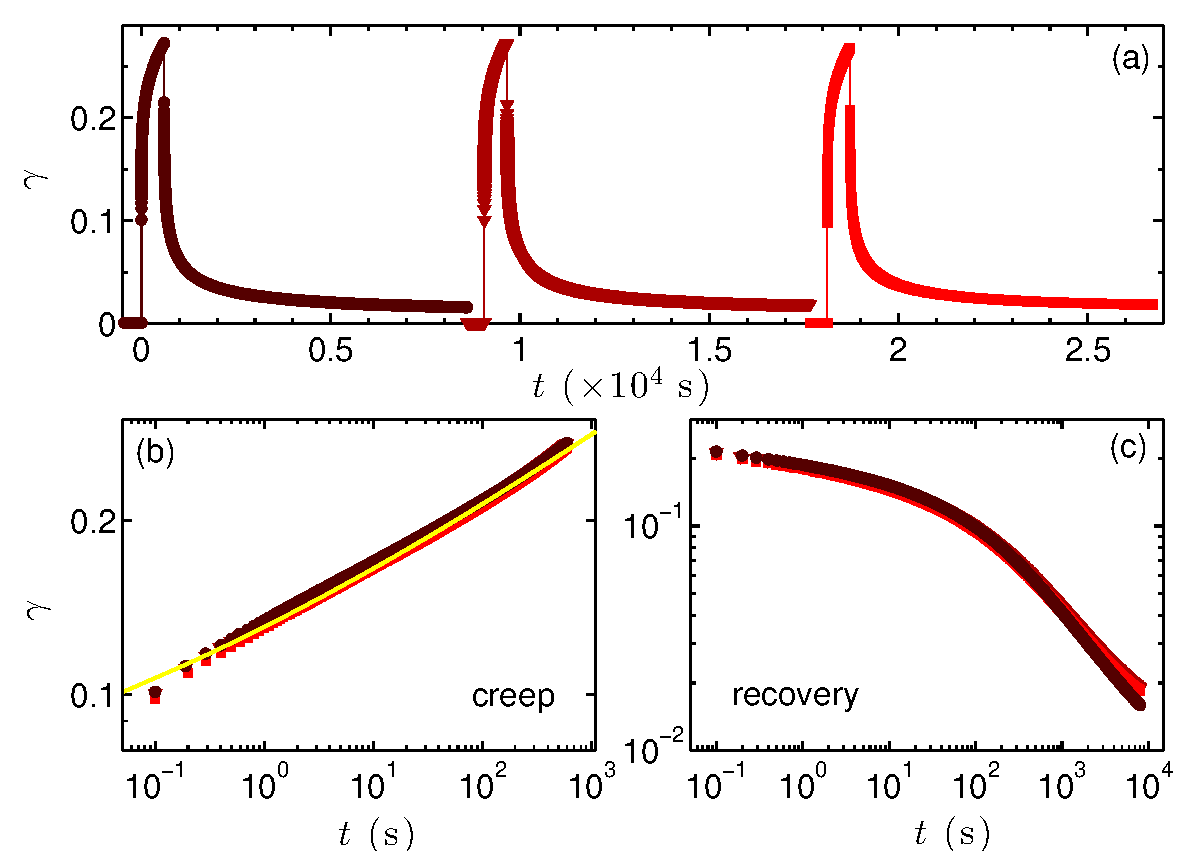
\includegraphics[width=8cm,clip]{SuppFig3.eps}
\caption{(color online) Three creep and recovery tests preformed successively in the primary creep regime on the same 4\%~wt. casein gel acidified with 1\%~wt. GDL. Prior to each test, the viscoelastic moduli are measured over 450~s under small amplitude oscillations around the reference position $\gamma=0$ (see Suppl. Fig.~\ref{suppfig4}). A constant stress $\sigma=100$~Pa is then applied for 600~s and finally the relaxation at $\sigma=0$ is followed over 8,000~s. (a)~Full strain response $\gamma(t)$ vs time. (b)~Superimposed strain responses during the three successive creep tests at $\sigma=100$~Pa and plotted in logarithmic scales as a function of the time since stress application. The yellow line is $\gamma(t)= 0.048+0.083 t^{0.15}$. (c)~Superimposed strain responses during the three recovery phases and plotted in logarithmic scales as a function of the time since stress is removed.
\label{suppfig3}}
\end{figure} 
%%%%%%%%%%%%

 %%%%%%%%%%%%
\begin{figure}
\centering
\includegraphics[width=6.5cm,clip]{SuppFig4.eps}
\caption{(color online) Linear viscoelastic moduli $G'$ (top) and $G''$ (bottom) as a function of frequency $f$ for a strain amplitude of 0.1\% recorded before each creep and recovery test shown in Suppl. Fig.~\ref{suppfig3}. The symbols \textcolor{red!25!black}{$\bullet$}, \textcolor{red!50!black}{$\blacktriangledown$} and \textcolor{red!75!black}{$\blacksquare$} respectively correspond to the first, second and third tests. Black lines are power laws $G'\sim G''\sim f^{0.15}$. 
\label{suppfig4}}
\end{figure} 
%%%%%%%%%%%%

Successive creep and recovery experiments performed on the same sample within the primary creep regime are presented in Supplemental Figures~\ref{suppfig3} and \ref{suppfig4}. When a stress of 100~Pa is applied at time $t=0$, an ``instantaneous'' elastic strain of about 10\% is recorded, followed by the slow Andrade creep already investigated in the main text and characterized by an exponent of 0.15 [Suppl. Fig.~\ref{suppfig3}(b)] that coincides with that of the frequency-dependence of both viscoelastic moduli $G'$ and $G''$ [Suppl. Fig.~\ref{suppfig4}]. When stress is removed at $t=600$~s, the strain drops by about 6\% and then slowly relaxes over several hours. After 8,000~s we observe that the initial strain is almost fully recovered: only a few percents are not (here 2\% out of a total maximum strain of 27\%).

Such an irrecoverable strain can be attributed either to viscous flow within the porous structure of the gel or to plastic events i.e. to local rupture of the gel network, and in the most general case to a combination of both. Interestingly, when the strain is reset to zero between two successive creep and recovery tests [i.e. the moving tool is moved back to its initial position, see the corresponding trace in Suppl. Fig.~\ref{suppfig3}(a)], the strain responses are indistinguishable [Suppl. Fig.~\ref{suppfig3}(b) and (c)]. If significant plastic deformation had occurred during the first loading--unloading cycle, one would have expected the second and third responses to the same cycle to differ significantly, e.g. through larger maximum strains or larger unrecoverable strains.

Finally Supplemental Figure 4 shows that both viscoelastic moduli $G'$ and $G''$ do not change significantly from one creep and recovery test to another and that their scaling with the frequency remains the same. This indicates that the gel microstructure is mostly undamaged by creep within the primary regime.

\begin{thebibliography}{}

\bibitem{Lucey:1998supp} J.A. Lucey and H. Singh, Food Res. Int. A {\bf 30}, 529--542 (1998).

\bibitem{Dickinson:2002supp} E. Dickinson and L.M. Merino, Food Hydrocolloid {\bf 16}, 321--331 (2002).

\end{thebibliography}

\end{document}
